\documentclass[11pt]{article}
\usepackage[review]{acl}
\usepackage{times}
\usepackage{latexsym}
\usepackage[T1]{fontenc}
\usepackage[utf8]{inputenc}
\usepackage{microtype}
\usepackage{inconsolata}
\usepackage{booktabs}
\usepackage{multirow}
\usepackage{amsmath}
\usepackage{amssymb}
\usepackage{graphicx}
\usepackage{xcolor}

\title{UCRID: Uncertainty-Aware Cascade Routing for Intent Detection and Out-of-Scope Detection}

\author{
Anonymous Authors \\
Affiliation \\
Address \\
\texttt{email@example.com}
}

\begin{document}
\maketitle

\begin{abstract}
Out-of-scope (OOS) detection is essential for task-oriented dialogue systems, but existing solutions typically face a trade-off between efficiency and robustness. Compact intent classifiers are fast and cheap, yet often unreliable on hard OOS cases, whereas large language models (LLMs) are more capable but too expensive to invoke for every query. We present \textbf{UCRID}, an uncertainty-aware cascade framework that combines a lightweight intent encoder, a dual-signal router, and candidate-constrained LLM arbitration. In Stage 1, a BERT-based encoder is trained with cross-entropy, supervised contrastive learning, and a boundary-aware loss to improve both intent discrimination and OOS separation in embedding space. In Stage 2, the model computes a fused uncertainty score from calibrated softmax entropy and prototype distance, and uses a dual-threshold policy to directly accept confident in-domain samples, directly reject obvious OOS samples, and forward only ambiguous cases. In Stage 3, an LLM performs final judgment only on the routed subset under a constrained candidate set. Experiments on CLINC150 and Banking77 show that UCRID achieves strong OOS performance while maintaining low LLM usage. Under the best current setting, UCRID reaches 84.31 OOS F1 on CLINC150 and 94.47 OOS F1 on Banking77 with only 8.1\% and 7.2\% LLM call rates, respectively. Ablation results further show that Stage-2 routing is indispensable, prototype distance is a stronger routing signal than entropy, and Stage-3 LLM arbitration remains necessary for the best end-to-end performance.
\end{abstract}

\section{Introduction}
Intent detection systems deployed in real applications must do more than classify supported intents accurately: they must also reject requests that fall outside the supported intent inventory. This out-of-scope (OOS) detection capability is particularly important in task-oriented assistants, customer service agents, and financial applications, where false acceptance may trigger incorrect downstream actions or degrade user trust.

Despite substantial progress on intent classification, OOS detection remains difficult because it is inherently an open-set problem. Samples that are semantically close to known intents may still be unsupported, while standard discriminative models are optimized primarily for closed-set classification. As a result, confidence-based heuristics often fail precisely on the boundary cases that matter most in deployment.

Current solutions tend to fall into one of two extremes. Lightweight encoders such as BERT are efficient and practical, but they often struggle with hard OOS cases near intent boundaries. Large language models (LLMs), in contrast, provide stronger semantic reasoning and broader generalization, but are too expensive to invoke for every user query. This motivates a hybrid strategy in which a compact encoder handles the majority of easy inputs and the LLM is reserved for a small subset of ambiguous cases.

We propose \textbf{UCRID}, a three-stage cascade framework for joint intent detection and OOS detection. In Stage 1, a BERT-based encoder is trained with cross-entropy, supervised contrastive learning, and a boundary-aware loss to improve both intent discrimination and OOS separation in embedding space. In Stage 2, a dual-signal router combines calibrated entropy and prototype distance to partition inputs into three regions: confident in-domain samples, obvious OOS samples, and ambiguous samples requiring escalation. In Stage 3, a candidate-constrained LLM performs final arbitration only on the routed subset.

The central premise of UCRID is that small models and LLMs should play distinct but complementary roles. The small model provides efficient broad coverage, the router provides uncertainty-aware triage, and the LLM serves as a high-capacity judge only where lightweight inference is no longer reliable. Under this design, the objective is not to maximize LLM usage, but to preserve strong OOS performance while keeping expensive inference tightly controlled.

Our contributions are as follows:
\begin{enumerate}
\item We propose a three-stage cascade framework that unifies lightweight intent classification, uncertainty-aware routing, and candidate-constrained LLM arbitration for efficient OOS detection.
\item We introduce a dual-signal routing mechanism that combines calibrated entropy and prototype distance with a dual-threshold decision policy.
\item We show through controlled ablations that Stage-2 routing is essential, prototype distance is the stronger routing signal, and Stage-3 LLM arbitration remains necessary for the best overall performance.
\item We provide an empirical comparison of open-source LLM backends within the same cascade, showing that the current \texttt{Qwen3-8B fixed} setup performs best in our pipeline.
\end{enumerate}

\section{Related Work}
\paragraph{Discriminative OOS detection.}
Early OOS detection methods largely rely on confidence thresholding or learned decision boundaries over discriminative intent encoders \citep{hendrycks2017baseline,zhang2021adb}. While efficient, such methods often fail on boundary OOS cases that remain close to known intents.

\paragraph{Representation learning and prototypes.}
Supervised contrastive learning and prototype-based modeling improve the geometry of the embedding space, making in-domain classes more compact and potentially more separable from OOS samples \citep{khosla2020supervised,khattak2020supcon}. These approaches are particularly relevant to OOS detection because they provide a natural distance-based signal for open-set recognition.

\paragraph{LLM-based intent and OOS detection.}
LLMs offer strong few-shot semantic reasoning, but full-query LLM inference is expensive and can be unstable under strict output constraints \citep{song2023chatgptintent,castillo2025lsr}. This makes them better suited as fallback judges than as universal first-pass classifiers in production settings.

\paragraph{Positioning of this work.}
UCRID combines these directions into a single deployment-oriented framework. Relative to pure small-model methods, it introduces selective LLM escalation rather than full-query inference. Relative to pure LLM approaches, it preserves efficiency by allowing lightweight classification to dominate the processing path. Relative to prior representation-learning methods, it uses prototype distance both as a training-time supervisory signal and as an inference-time routing signal.

\section{Method}
\subsection{Problem Definition}
Let $\mathcal{Y}_{ID}=\{1,\dots,C\}$ be the set of in-domain intents and let $\text{OOS}$ denote the out-of-scope label. Given a user utterance $u$, the system must either assign an intent from $\mathcal{Y}_{ID}$ or reject the utterance as OOS.

\subsection{Overview}
UCRID contains three stages:
\begin{enumerate}
\item \textbf{Stage 1}: a BERT-based encoder outputs logits and hidden representations.
\item \textbf{Stage 2}: a dual-signal router computes uncertainty and decides whether to accept, reject, or escalate.
\item \textbf{Stage 3}: an LLM arbitrates only the ambiguous cases under a restricted candidate set.
\end{enumerate}

This decomposition is deliberately asymmetric: the small model processes every query, while the LLM is reserved for a minority of hard cases. The router is therefore the key mediator between efficiency and robustness.

\subsection{Stage 1: Multi-Objective Intent Encoder}
The Stage-1 encoder is trained with:
\begin{equation}
\mathcal{L} = \mathcal{L}_{CE} + \lambda_s \mathcal{L}_{SupCon} + \lambda_b \mathcal{L}_{Boundary}.
\end{equation}

$\mathcal{L}_{CE}$ ensures standard classification performance. $\mathcal{L}_{SupCon}$ improves class-wise compactness in embedding space. $\mathcal{L}_{Boundary}$ explicitly pushes OOS samples away from in-domain prototypes.

For each in-domain class $c$, we define a prototype:
\begin{equation}
p_c = \frac{1}{N_c}\sum_{i:y_i=c} h_i.
\end{equation}

For an OOS sample $x$, the boundary-aware term is:
\begin{equation}
\mathcal{L}_{Boundary} = \max(0, \Delta - d(h_x, p_{c^*})),
\end{equation}
where $c^*=\arg\min_c d(h_x,p_c)$ and $d(\cdot,\cdot)$ is Euclidean distance.

The role of the boundary-aware term is important. It does not merely improve classification margins; it explicitly reshapes the embedding space so that OOS samples are less likely to occupy regions close to known intent clusters. This is what later makes prototype distance a meaningful routing signal at inference time.

\subsection{Stage 2: Dual-Signal Uncertainty Router}
For each sample $u$, the router computes:
\begin{equation}
H(u) = -\sum_y p(y|u)\log p(y|u),
\end{equation}
\begin{equation}
d_{min}(u)=\min_c ||h_u-p_c||_2.
\end{equation}

After calibration and normalization, the fused uncertainty score is:
\begin{equation}
s(u)=\alpha H_{norm}(u)+(1-\alpha)d_{norm}(u).
\end{equation}

The dual-threshold decision rule is:
\begin{itemize}
\item if $s(u)\le \tau_{accept}$, accept the Stage-1 top-1 intent;
\item if $s(u)\ge \tau_{reject}$ and $d_{min}(u)>\Delta$, directly reject as OOS;
\item otherwise, send the sample to the LLM.
\end{itemize}

Unlike a single-threshold design, this policy creates three operationally distinct regions: a confident in-domain region, a clear OOS region, and an ambiguity band. This three-way partition is central to making the cascade practical.

\subsection{Stage 3: Candidate-Constrained LLM Arbitration}
For routed queries, the LLM receives a small candidate list from the Stage-1 top-$k$ intents together with intent descriptions and few-shot examples. The LLM is asked to output either one candidate intent or \texttt{OOS}. This restricted candidate space improves stability and lowers risk compared with unconstrained full-label prompting.

In the current best configuration, the system adopts a conservative \texttt{oos\_only} acceptance policy, meaning that the LLM is primarily trusted to issue valid OOS corrections rather than unrestricted intent substitutions. This reduces the risk of noisy label overrides while still allowing the cascade to recover hard OOS cases.

\section{Experimental Setup}
\subsection{Datasets}
We evaluate on CLINC150, Banking77, and HINT3-v2. CLINC150 provides a standard benchmark with 150 in-domain intents and an explicit OOS category \citep{larson2019clinc150}. Banking77 offers a fine-grained banking intent benchmark under the current project-specific OOS evaluation pipeline \citep{casanueva2020banking77}. HINT3-v2 provides three business-specific subsets (\texttt{curekart}, \texttt{sofmattress}, and \texttt{powerplay11}) that allow us to probe cross-domain transfer under a more deployment-oriented data condition. For HINT3-v2, we convert the dataset into the UCRID JSON format required by our pipeline and treat \texttt{NO\_NODES\_DETECTED} as the OOS label.

\subsection{Metrics}
We report overall accuracy, in-domain accuracy, OOS precision, OOS recall, OOS F1, and LLM call rate. Here, overall accuracy is computed over all test samples, whereas in-domain accuracy is computed only on the subset of in-domain examples.

\subsection{Implementation Notes}
The best current end-to-end system uses \texttt{Qwen3-8B fixed + oos\_only} as the Stage-3 backend. We also compare \texttt{Qwen2-7B} and \texttt{Mixtral-8x7B-v0.1} within the same cascade. Importantly, our experimental discussion distinguishes strictly between controlled comparisons under the same project pipeline and contextual comparisons to prior work under heterogeneous protocols.

\section{Main Results}
\subsection{Best End-to-End Results}
\begin{figure*}[t]
\centering
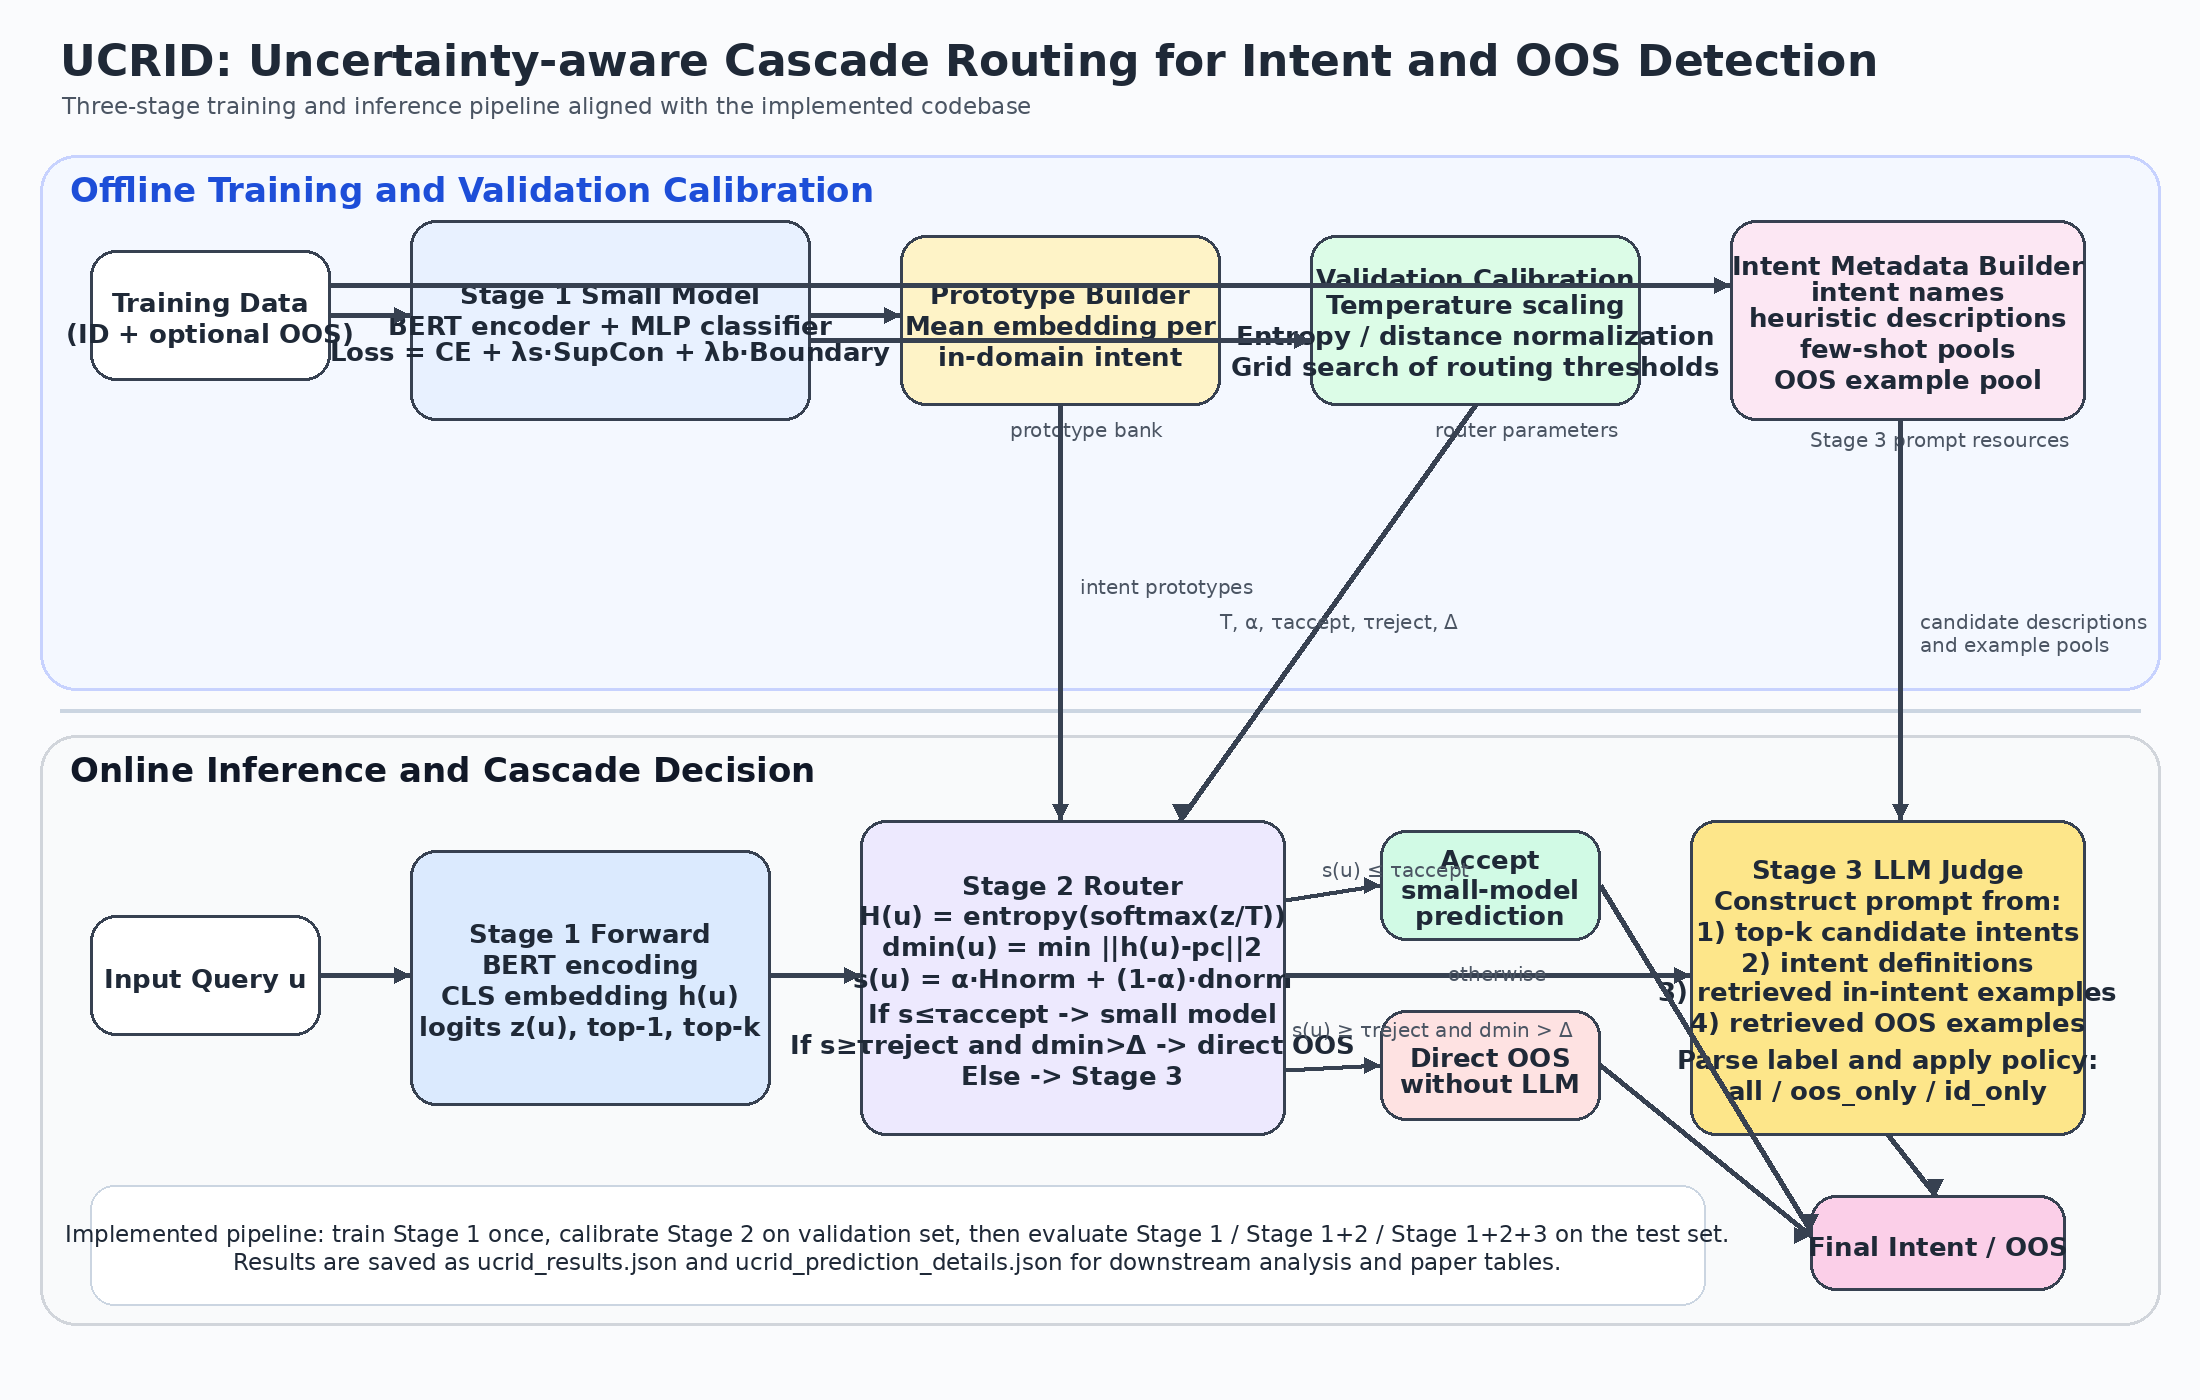
\includegraphics[width=0.95\textwidth]{figures/ucrid_pipeline_diagram_20260321.png}
\caption{Overview of UCRID. A lightweight encoder first processes every query. The dual-signal router then separates confident in-domain samples, obvious OOS samples, and ambiguous samples that are escalated to Stage-3 LLM arbitration.}
\label{fig:ucrid_pipeline}
\end{figure*}

\begin{figure*}[t]
\centering
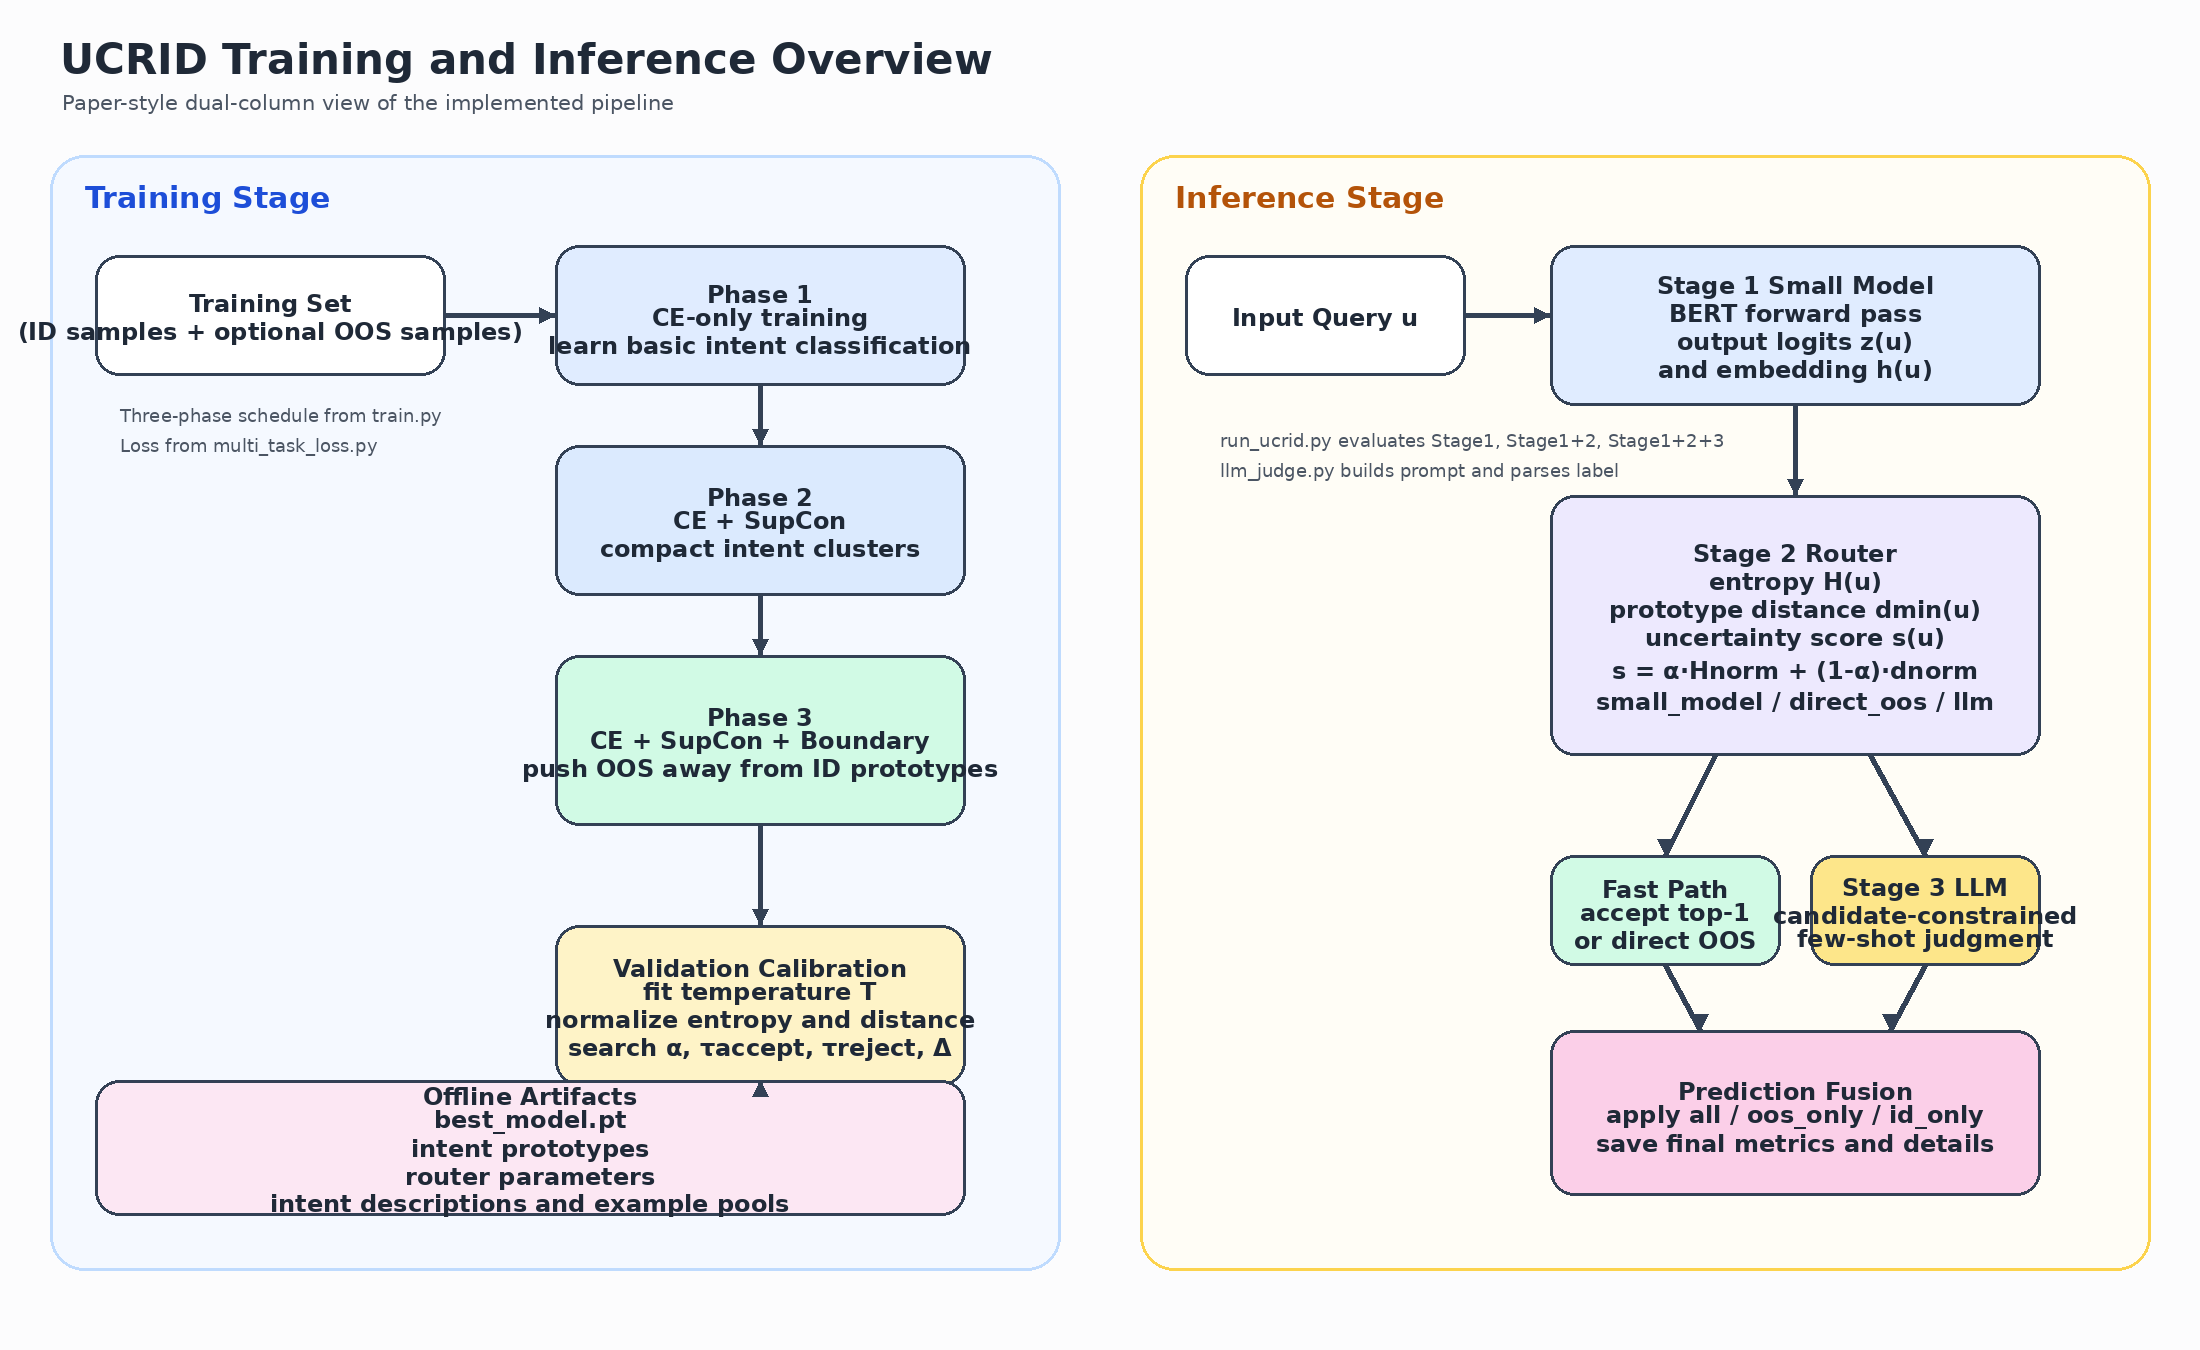
\includegraphics[width=0.95\textwidth]{figures/ucrid_dual_column_train_infer_20260321.png}
\caption{Two-view illustration of UCRID. Left: training phase with cross-entropy, supervised contrastive loss, and boundary-aware loss. Right: inference phase with uncertainty-aware routing and candidate-constrained LLM judgment.}
\label{fig:train_infer}
\end{figure*}

\begin{table}[t]
\centering
\caption{Best end-to-end results of UCRID.}
\label{tab:main_results}
\begin{tabular}{lcccccc}
\toprule
Dataset & Acc. & ID Acc. & OOS Prec. & OOS Rec. & OOS F1 & LLM Rate \\
\midrule
CLINC150 & 92.40 & 95.91 & 93.76 & 76.60 & 84.31 & 8.1 \\
Banking77 & 92.65 & 92.44 & 94.95 & 94.00 & 94.47 & 7.2 \\
\bottomrule
\end{tabular}
\end{table}

UCRID achieves strong OOS detection on both benchmarks while keeping LLM usage low. This indicates that the proposed small-model-first cascade design is effective in practice. Figure~\ref{fig:ucrid_pipeline} shows the overall cascade, while Figure~\ref{fig:train_infer} separates the training and inference views of the full system.

\subsection{LLM Backend Comparison}
\begin{table}[t]
\centering
\caption{Stage-3 backend comparison on CLINC150.}
\label{tab:clinc_llm_compare}
\begin{tabular}{lcccc}
\toprule
Backend & Accuracy & ID Acc. & OOS F1 & LLM Rate \\
\midrule
Qwen2-7B baseline & 90.51 & \textbf{95.96} & 77.65 & 8.1 \\
Qwen3-8B fixed & \textbf{92.40} & 95.91 & \textbf{84.31} & 8.1 \\
Mixtral-8x7B-v0.1 & 91.02 & 95.91 & 79.45 & 8.1 \\
\bottomrule
\end{tabular}
\end{table}

\begin{table}[t]
\centering
\caption{Stage-3 backend comparison on Banking77.}
\label{tab:banking_llm_compare}
\begin{tabular}{lcccc}
\toprule
Backend & Accuracy & ID Acc. & OOS F1 & LLM Rate \\
\midrule
Qwen2-7B baseline & 92.60 & 92.37 & 94.00 & 7.2 \\
Qwen3-8B fixed & \textbf{92.65} & 92.44 & \textbf{94.47} & 7.2 \\
Mixtral-8x7B-v0.1 & 91.76 & \textbf{92.47} & 91.04 & 7.2 \\
\bottomrule
\end{tabular}
\end{table}

Among the three tested open-source backends, \texttt{Qwen3-8B fixed} yields the strongest and most stable performance in the current pipeline. Notably, the backend comparisons also show why overall accuracy and in-domain accuracy should be reported separately: some backends remain competitive on in-domain accuracy while still underperforming substantially on OOS F1. The gap is especially visible on CLINC150, suggesting that this dataset is more sensitive to output controllability, OOS formatting consistency, and constrained label following.

\subsection{Additional Generalization Results on HINT3-v2}
\begin{table*}[t]
\centering
\caption{Additional end-to-end generalization results on HINT3-v2 using the same \texttt{Qwen3-8B + oos\_only} pipeline.}
\label{tab:hint3_results}
\begin{tabular}{lcccccc}
\toprule
Subset & Acc. & ID Acc. & OOS Prec. & OOS Rec. & OOS F1 & LLM Rate \\
\midrule
curekart & 67.09 & 47.14 & 66.36 & 84.27 & 74.25 & 25.47 \\
sofmattress & 49.21 & 24.26 & 44.03 & 93.04 & 59.78 & 18.61 \\
powerplay11 & 65.65 & 23.48 & 79.93 & 84.97 & 82.37 & 32.44 \\
Macro average & 60.65 & 31.63 & 63.44 & 87.43 & 72.13 & 25.51 \\
\bottomrule
\end{tabular}
\end{table*}

The HINT3-v2 results reveal a different operating regime from CLINC150 and Banking77. Although UCRID still maintains strong OOS recall across all three subsets, in-domain accuracy drops substantially, especially on \texttt{sofmattress} and \texttt{powerplay11}. This pattern suggests that HINT3-v2 imposes a harsher open-set condition in which many samples are easier to reject as unsupported than to map precisely to the correct in-domain intent. Correspondingly, the router behaves more conservatively, with a larger fraction of traffic going to direct OOS rejection and a higher LLM call rate than on the main benchmarks. From a generalization standpoint, these findings are still encouraging: they show that the proposed cascade preserves robust OOS sensitivity under industrial-style domain shift, while also making clear that fine-grained in-domain intent resolution remains the main bottleneck outside cleaner benchmark distributions.

\section{Ablation Study}
\begin{figure}[t]
\centering
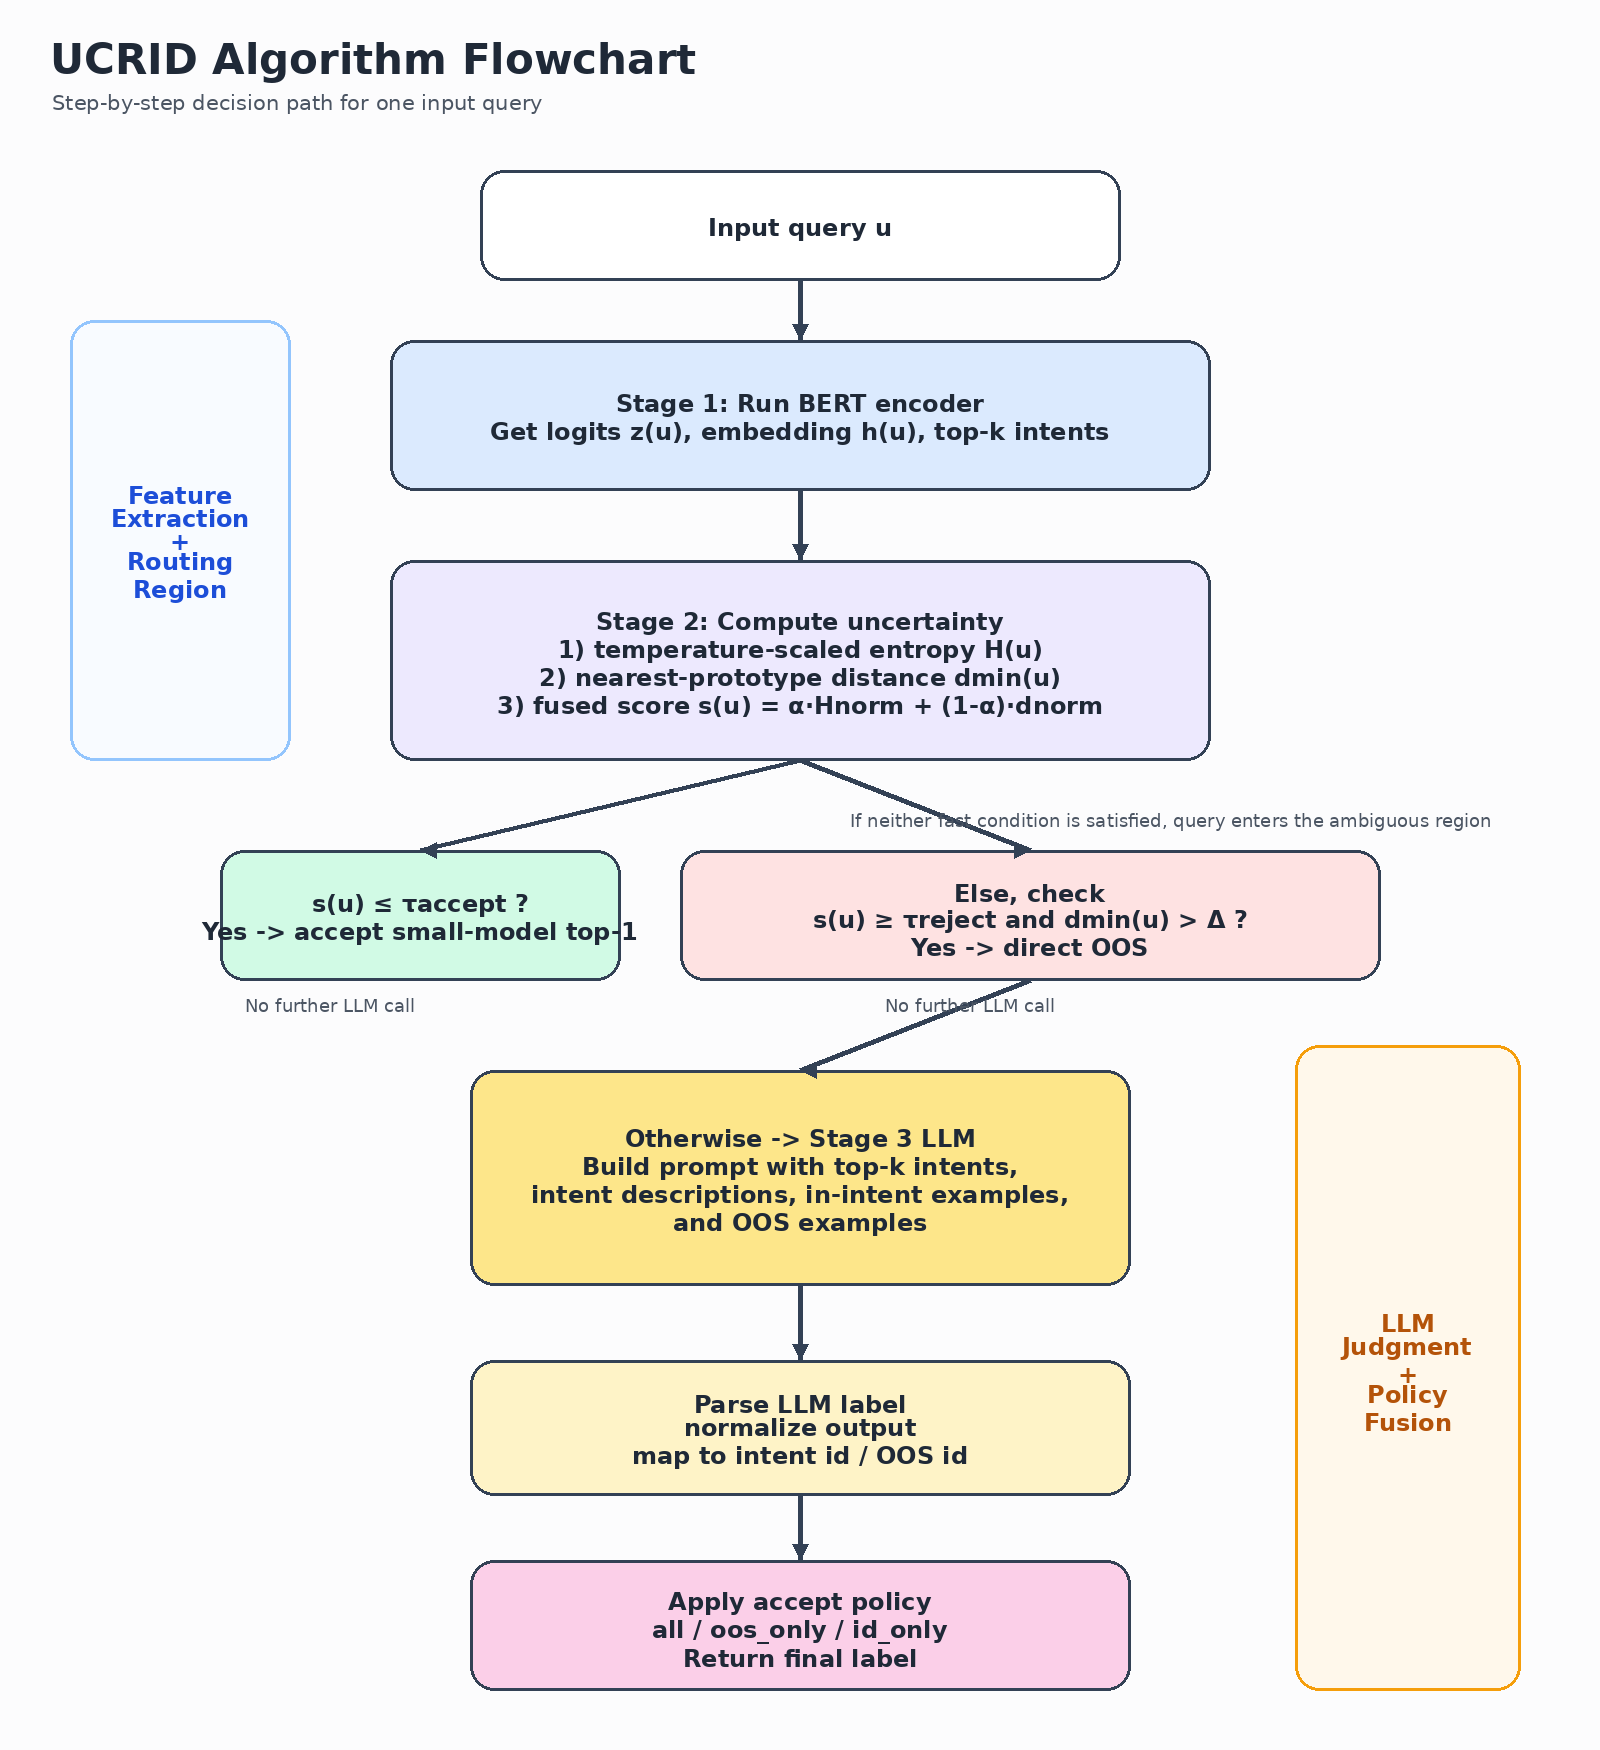
\includegraphics[width=0.48\textwidth]{figures/ucrid_algorithm_flowchart_20260321.png}
\caption{Algorithmic flow of UCRID inference. The router computes entropy and prototype distance, applies dual-threshold decisions, and forwards only ambiguous cases to the LLM.}
\label{fig:algorithm_flow}
\end{figure}

\begin{figure}[t]
\centering
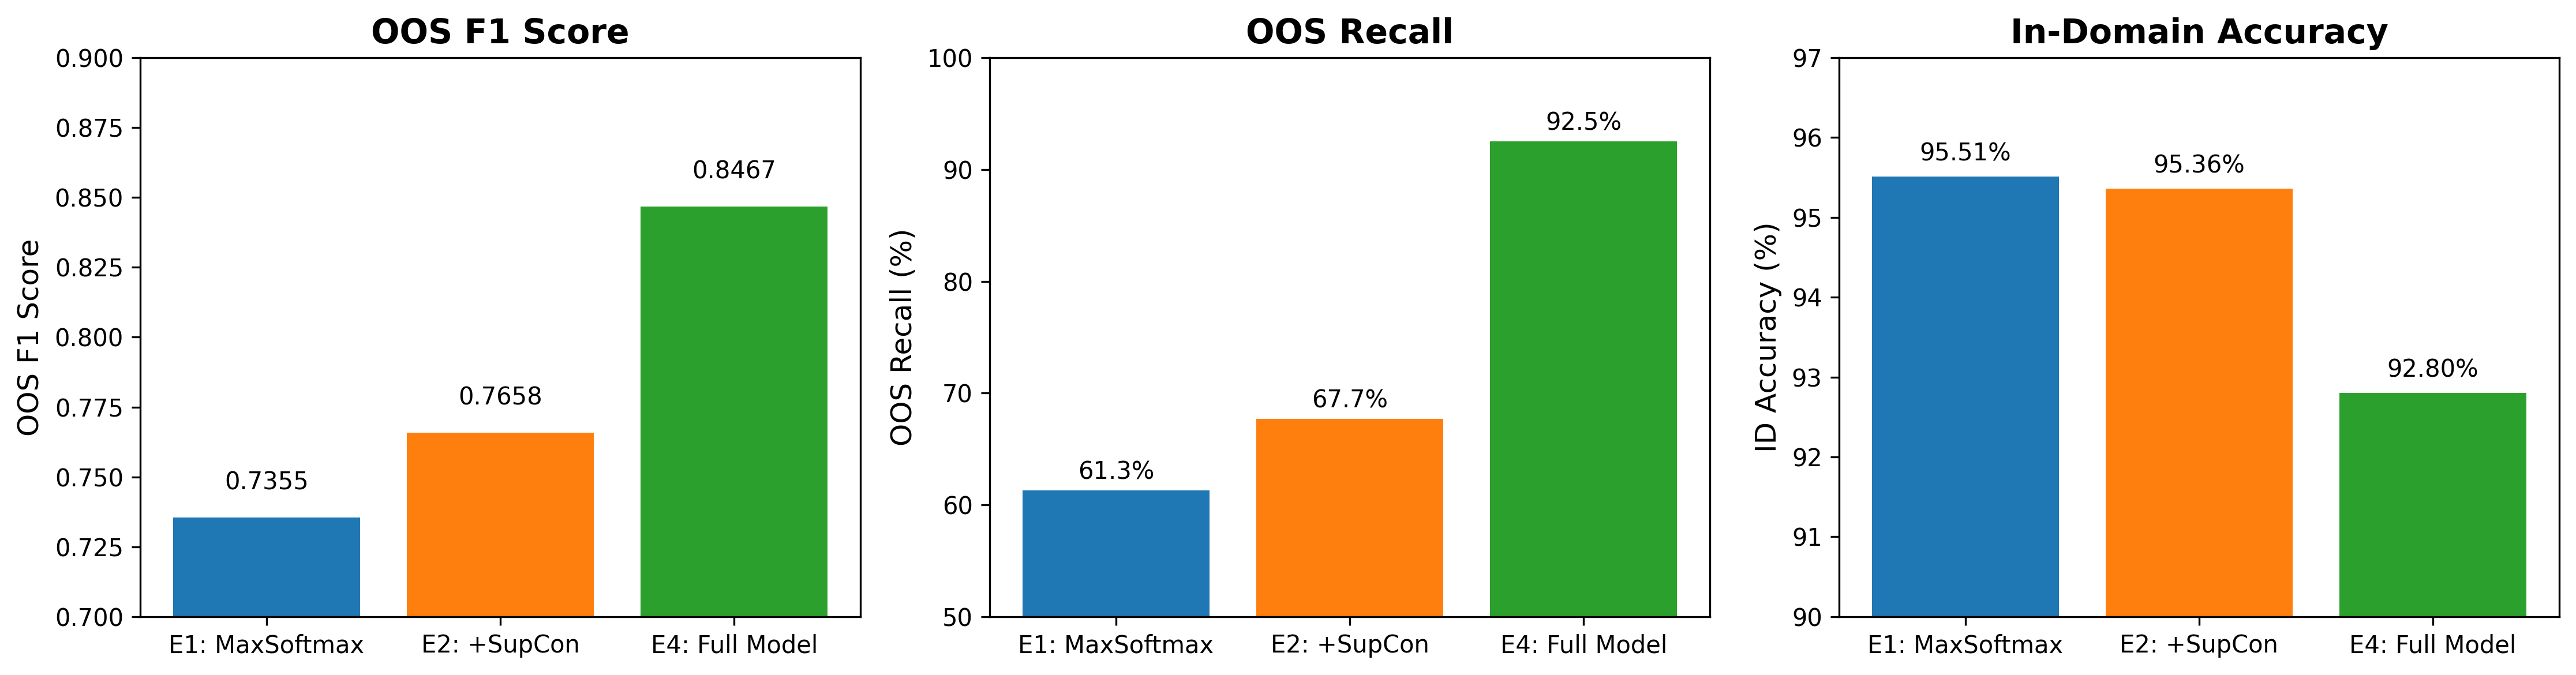
\includegraphics[width=0.48\textwidth]{figures/ablation_chart.png}
\caption{Ablation comparison on CLINC150 and Banking77. Prototype distance contributes more than entropy, while the full UCRID cascade achieves the best final OOS F1.}
\label{fig:ablation_chart}
\end{figure}

\begin{table*}[t]
\centering
\caption{Ablation results on CLINC150 and Banking77.}
\label{tab:ablation}
\begin{tabular}{llcccccc}
\toprule
Dataset & Method & Acc. & ID Acc. & OOS Prec. & OOS Rec. & OOS F1 & LLM Rate \\
\midrule
\multirow{5}{*}{CLINC150}
& Stage1 only & 86.35 & 96.07 & 95.73 & 42.60 & 58.96 & - \\
& Stage1+2 (full router) & 89.55 & 95.96 & 93.82 & 60.70 & 73.71 & 8.1 \\
& w/o distance (entropy-only) & 89.11 & 95.98 & 94.33 & 58.20 & 71.99 & 5.9 \\
& w/o entropy (distance-only) & 91.07 & 95.76 & 91.50 & 70.00 & 79.32 & 9.6 \\
& Full UCRID & \textbf{92.40} & 95.91 & 93.76 & \textbf{76.60} & \textbf{84.31} & 8.1 \\
\midrule
\multirow{5}{*}{Banking77}
& Stage1 only & 79.78 & \textbf{92.73} & 0.00 & 0.00 & 0.00 & - \\
& Stage1+2 (full router) & 89.94 & 92.47 & 95.38 & 74.40 & 83.60 & 7.2 \\
& w/o distance (entropy-only) & 89.61 & 92.53 & \textbf{95.72} & 71.60 & 81.92 & 6.2 \\
& w/o entropy (distance-only) & 91.17 & 92.34 & 91.50 & 84.00 & 87.59 & 11.9 \\
& Full UCRID & \textbf{92.65} & 92.44 & 94.95 & \textbf{94.00} & \textbf{94.47} & 7.2 \\
\bottomrule
\end{tabular}
\end{table*}

The ablation study supports three conclusions. First, Stage-2 routing is essential, since Stage1-only performance is substantially weaker on both datasets. Second, prototype distance is the stronger routing signal, as the distance-only variant consistently outperforms the entropy-only variant in OOS F1. Third, Stage-3 LLM arbitration remains necessary for the best final results, showing that routing and LLM judgment are complementary rather than redundant. Figure~\ref{fig:algorithm_flow} summarizes the inference logic, and Figure~\ref{fig:ablation_chart} visualizes the main ablation trend.

\section{Discussion}
Prototype distance outperforms entropy because it directly measures whether a sample lies near any known intent cluster in embedding space. Entropy reflects classifier hesitation, but does not fully capture geometric separation. A sample may receive a relatively confident but still incorrect prediction while remaining far from all known prototypes. This explains why the distance-only router is stronger than the entropy-only variant in both datasets.

It is also important that the best result comes from the \texttt{Qwen3-8B fixed} configuration rather than the earlier raw \texttt{Qwen3-8B} run. This improvement is largely due to engineering alignment: better prompt constraints, output parsing robustness, and a more stable integration policy increased the proportion of valid Stage-3 decisions that could be accepted by the cascade. This observation is practically important, because it shows that backend quality in hybrid systems depends not only on raw model capability, but also on interface controllability.

\section{Limitations}
This work has several limitations. First, not all literature comparisons are directly numerical because existing studies use different known-intent splits, datasets, or metrics. Second, the current analysis focuses on a limited set of open-source LLM backends, and broader evaluation across stronger proprietary models would provide a fuller picture. Third, Banking77 requires project-specific OOS adaptation, so additional validation on naturally OOS-rich benchmarks would further strengthen the claims. Finally, the current prototype representation is based on class means and may be extended with richer prototype structures or dynamic prototype refinement in future work.

\section{Conclusion}
We presented UCRID, a three-stage cascade framework that combines a lightweight encoder, uncertainty-aware routing, and candidate-constrained LLM arbitration for intent detection and OOS detection. The results show that strong OOS performance can be achieved with low LLM call rates, making the cascade practical for deployment-oriented systems. Ablation studies confirm that Stage-2 routing is essential, prototype distance is the dominant routing signal, and Stage-3 LLM arbitration delivers the final performance gains. More broadly, the results suggest that effective OOS detection should be treated not as a choice between compact encoders and LLMs, but as a coordinated cascade in which both components serve different and complementary functions.

\section*{Ethics Statement}
This work studies intent detection and OOS detection for dialogue systems. Potential risks include biased model behavior, unsafe rejection or acceptance of user requests, and privacy concerns when LLM backends are used. In practical deployment, sensitive user data should be protected, and routed LLM usage should comply with security and privacy policies.

\section*{Acknowledgments}
Acknowledgments omitted for anonymous review.

\bibliographystyle{acl_natbib}
\bibliography{UCRID_references_20260325}

\end{document}
